%!TEX root = ../thesis.tex
% Plotting the orbital plots for each target

\todo{change RV scale for hd4747 orbit}
\todo{Fix plot titles}
\begin{figure}
    \centering
    \begin{tabular}{cc}
        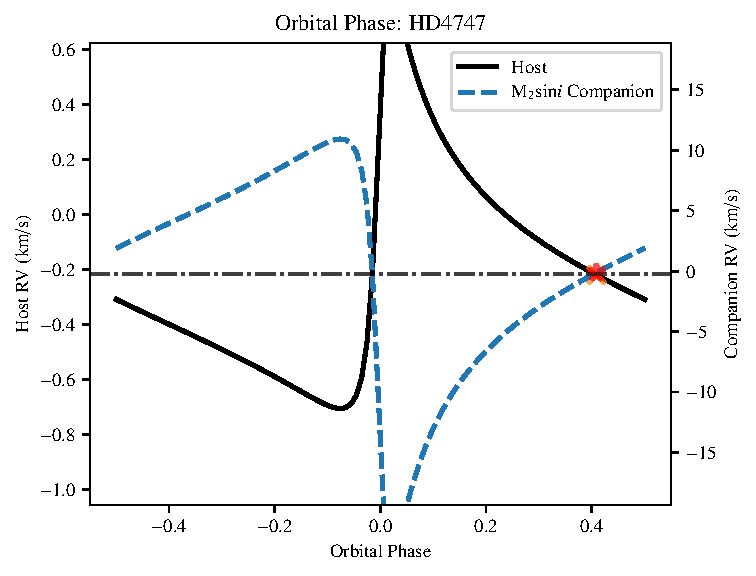
\includegraphics[width=0.45\linewidth]{figures/direct-recovery/orbital-plots/HD4747_orbital_phase.pdf}& 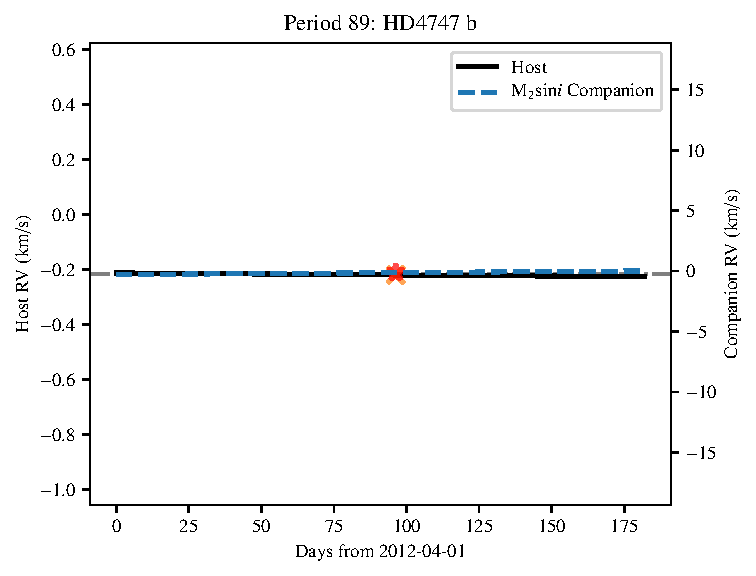
\includegraphics[width=0.45\linewidth]{figures/direct-recovery/orbital-plots/HD4747_p89.pdf}\\
    \end{tabular}
    \caption{RV orbital single companion Keplerian for the {HD\,4747}. The left hand plot shows the RV curve for one full orbit while the right hand panel shows the RV curve over 6 months (Period 89). The solid black line indicates the RV of the host star (with scale on the left), while the blue dashed line indicates the RV of the companion (with scale on the right axis). The orange crosses and red stars indicate the times at which observations were obtained for the target, for the host and companion respectively.}
    \label{fig:hd4747p89}
\end{figure}

\begin{figure}
    \centering
    \begin{tabular}{cc}
        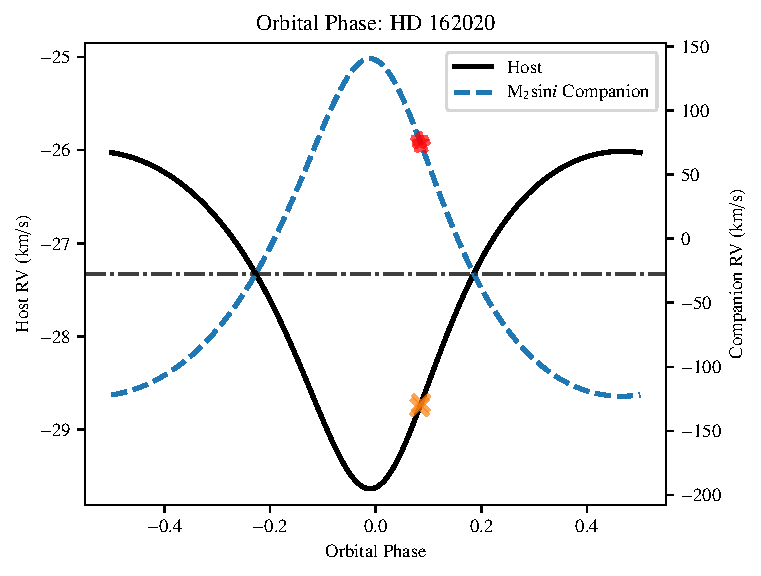
\includegraphics[width=0.45\linewidth]{figures/direct-recovery/orbital-plots/HD162020_orbital_phase.pdf}&
        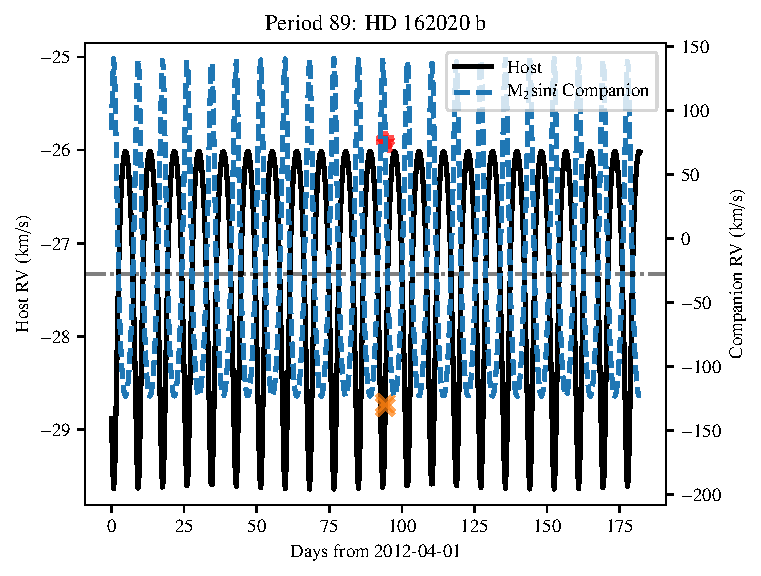
\includegraphics[width=0.45\linewidth]{figures/direct-recovery/orbital-plots/HD162020_p89.pdf}\\
    \end{tabular}
    \caption{Same as \fref{fig:hd4747p89} but for {HD\,162020}.}
    \label{fig:hd162020p89}
\end{figure}

\begin{figure}
    \centering
    \begin{tabular}{cc}
        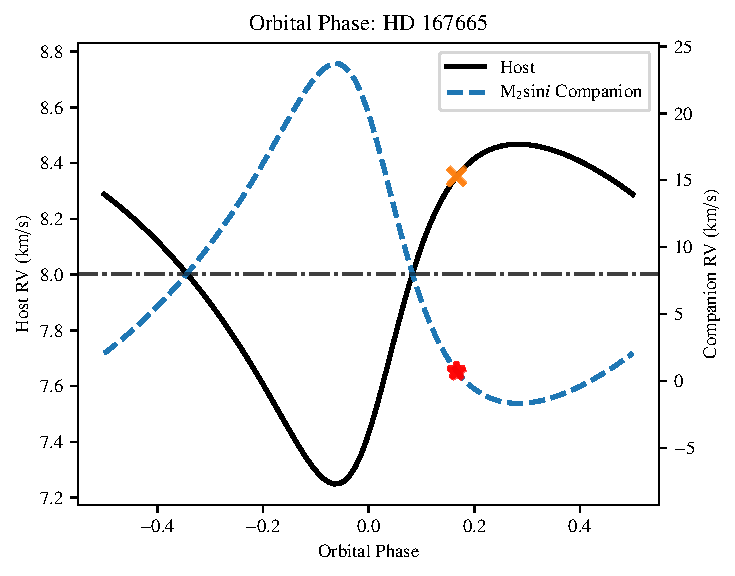
\includegraphics[width=0.45\linewidth]{figures/direct-recovery/orbital-plots/HD167665_orbital_phase.pdf}&
        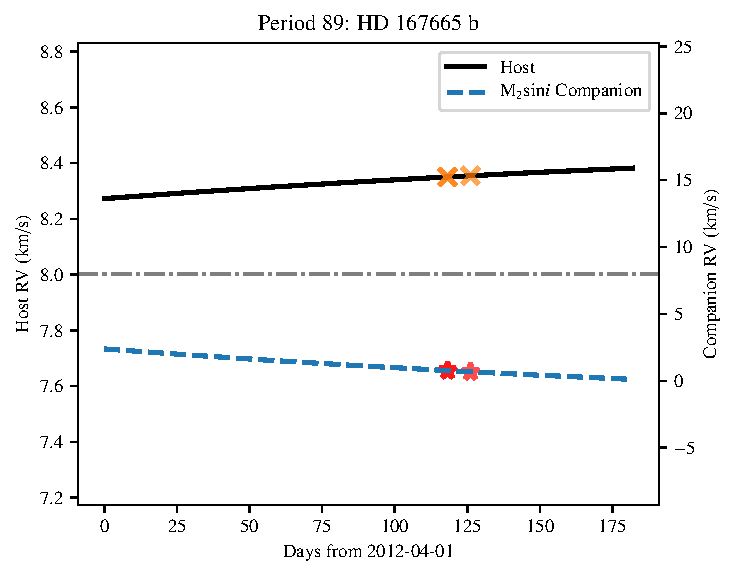
\includegraphics[width=0.45\linewidth]{figures/direct-recovery/orbital-plots/HD167665_p89.pdf}\\
    \end{tabular}
    \caption{Same as \fref{fig:hd4747p89} but for {HD\,167665}.}
    \label{fig:hd167665p89}
\end{figure}

\begin{figure}
    \centering
    \begin{tabular}{cc}
        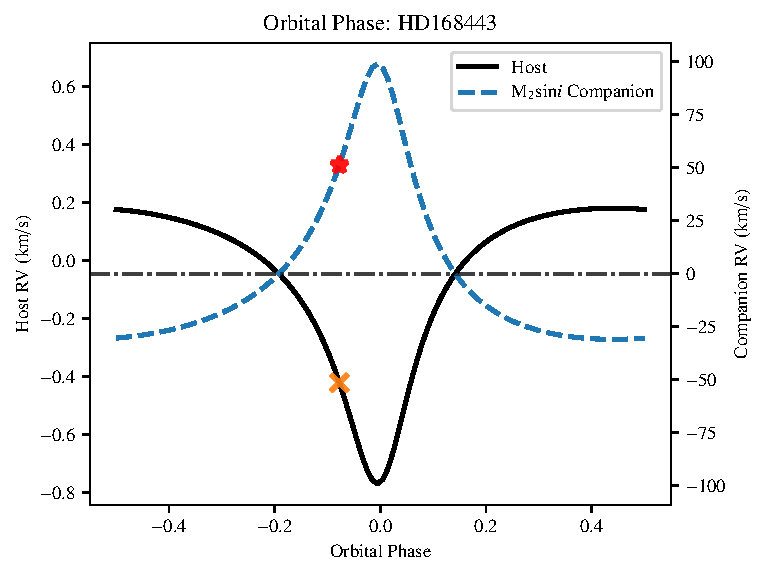
\includegraphics[width=0.45\linewidth]{figures/direct-recovery/orbital-plots/HD168443b_orbital_phase.pdf}&
        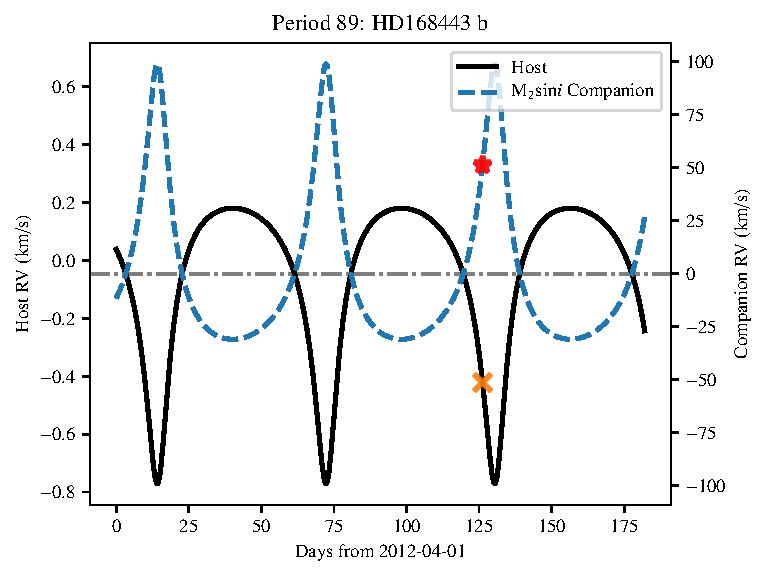
\includegraphics[width=0.45\linewidth]{figures/direct-recovery/orbital-plots/HD168443b_p89.pdf}\\
    \end{tabular}
    \caption{Same as \fref{fig:hd4747p89} but for {HD\,168443}b. Analysed as if this was a single companion.}
    \label{fig:hd168443bp89}
\end{figure}


\begin{figure}
    \centering
    \begin{tabular}{cc}
        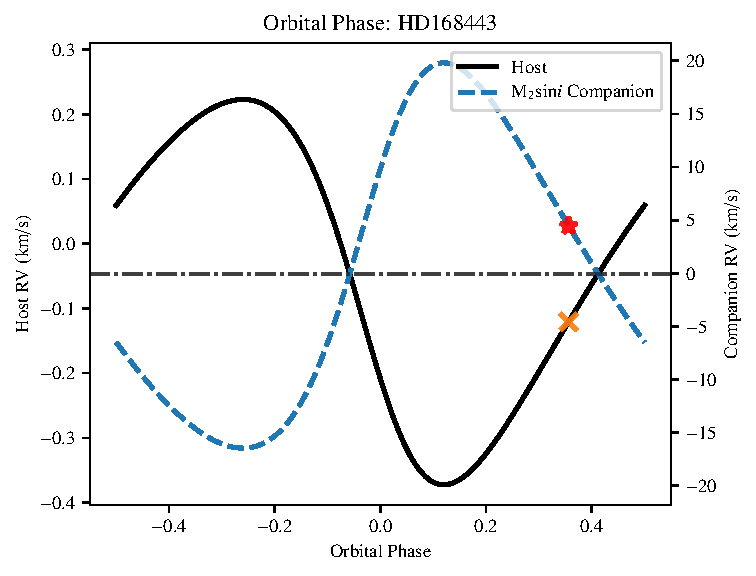
\includegraphics[width=0.45\linewidth]{figures/direct-recovery/orbital-plots/HD168443c_orbital_phase.pdf}&
        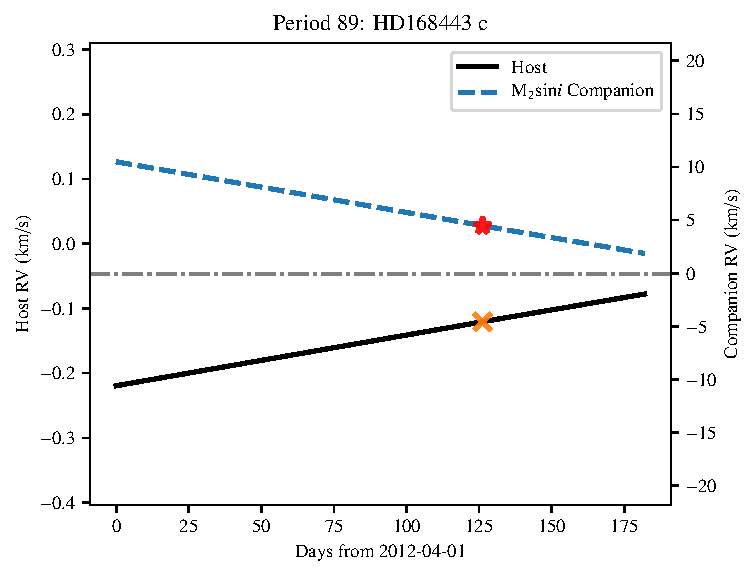
\includegraphics[width=0.45\linewidth]{figures/direct-recovery/orbital-plots/HD168443c_p89.pdf}\\
    \end{tabular}
    \caption{Same as \fref{fig:hd4747p89} but for {HD\,168443}c. Analysed as if this was a single companion.}
    \label{fig:hd168443cp89}
\end{figure}

\begin{figure}
    \centering
    \begin{tabular}{cc}
        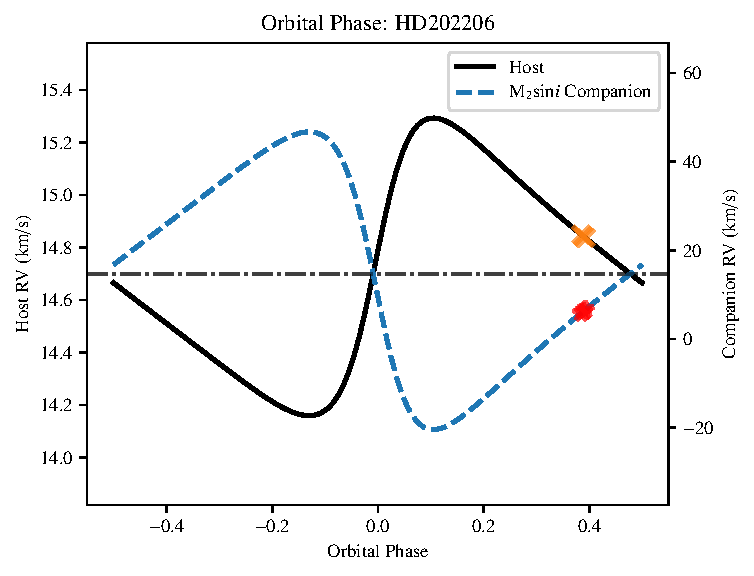
\includegraphics[width=0.45\linewidth]{figures/direct-recovery/orbital-plots/HD202206B_orbital_phase.pdf}&
        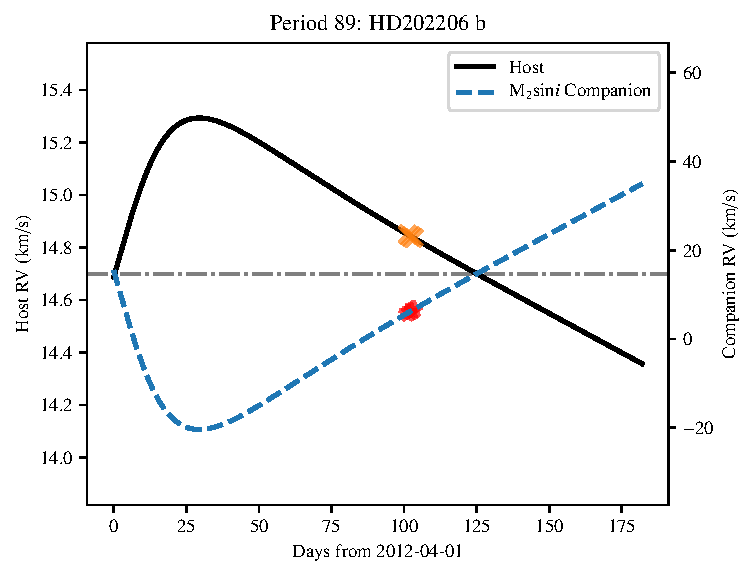
\includegraphics[width=0.45\linewidth]{figures/direct-recovery/orbital-plots/HD202206B_p89.pdf}\\
    \end{tabular}
    \caption{Same as \fref{fig:hd4747p89} but for {HD\,202206}B. Analysed as if this was a single companion.}
    \label{fig:hd202206bp89}
\end{figure}

\begin{figure}
    \centering
    \begin{tabular}{cc}
        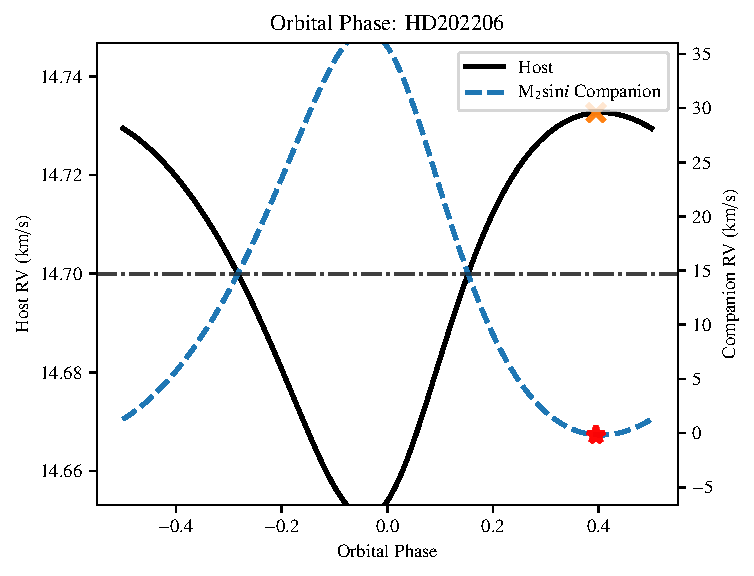
\includegraphics[width=0.45\linewidth]{figures/direct-recovery/orbital-plots/HD202206c_orbital_phase.pdf}&
        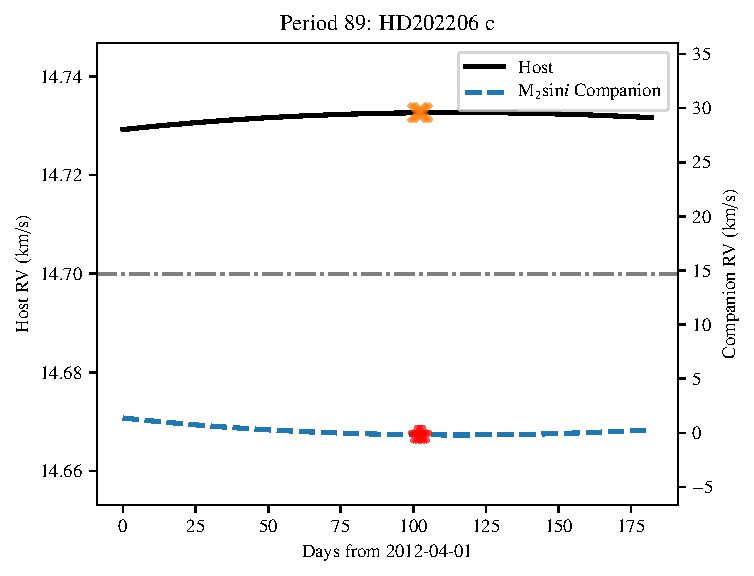
\includegraphics[width=0.45\linewidth]{figures/direct-recovery/orbital-plots/HD202206c_p89.pdf}\\
    \end{tabular}
    \caption{Same as \fref{fig:hd4747p89} but for {HD\,202206}c. Analysed as if this was a single companion. }
    \label{fig:hd202206cp89}
\end{figure}

\begin{figure}
    \centering
    \begin{tabular}{cc}
        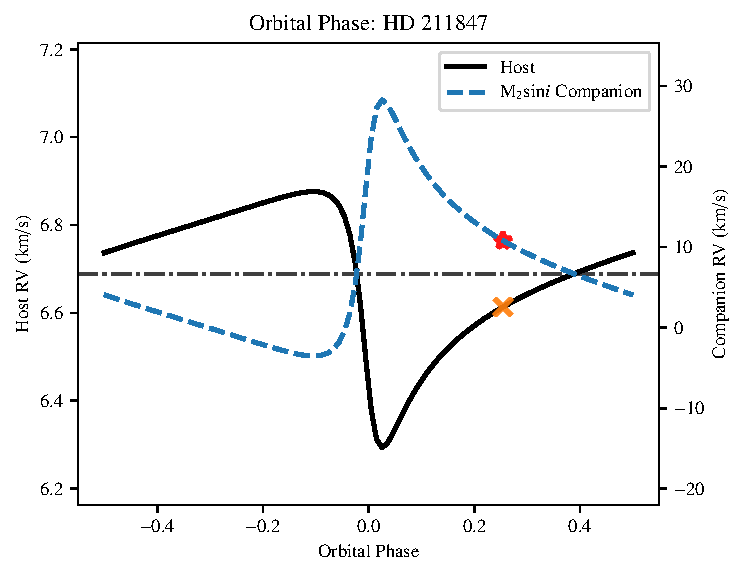
\includegraphics[width=0.45\linewidth]{figures/direct-recovery/orbital-plots/HD211847_orbital_phase.pdf}&
        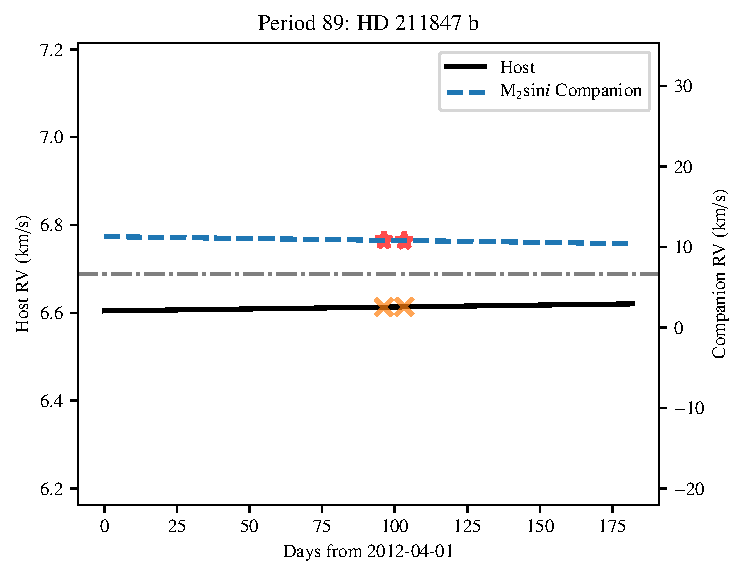
\includegraphics[width=0.45\linewidth]{figures/direct-recovery/orbital-plots/HD211847_p89.pdf}\\
    \end{tabular}
    \caption{Same as \fref{fig:hd4747p89} but for {HD\,211847}.}
    \label{fig:hd211847p89}
\end{figure}

\begin{figure}
    \centering
    \begin{tabular}{cc}
        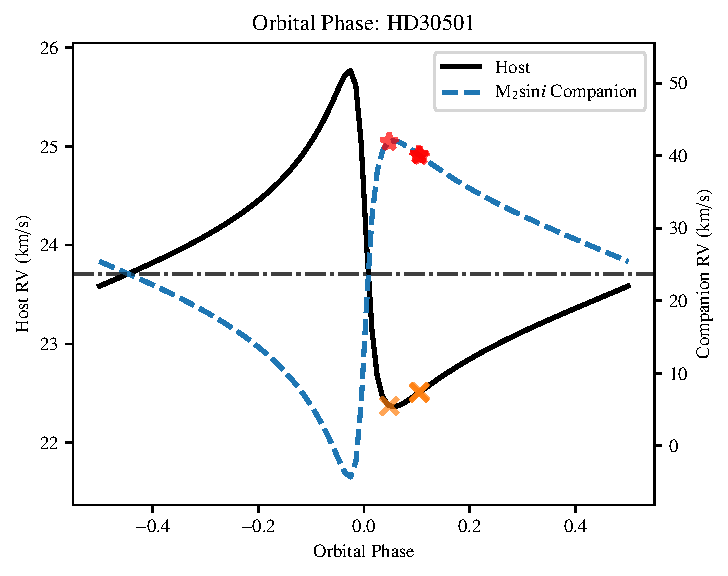
\includegraphics[width=0.45\linewidth]{figures/direct-recovery/orbital-plots/HD30501_orbital_phase.pdf}&
        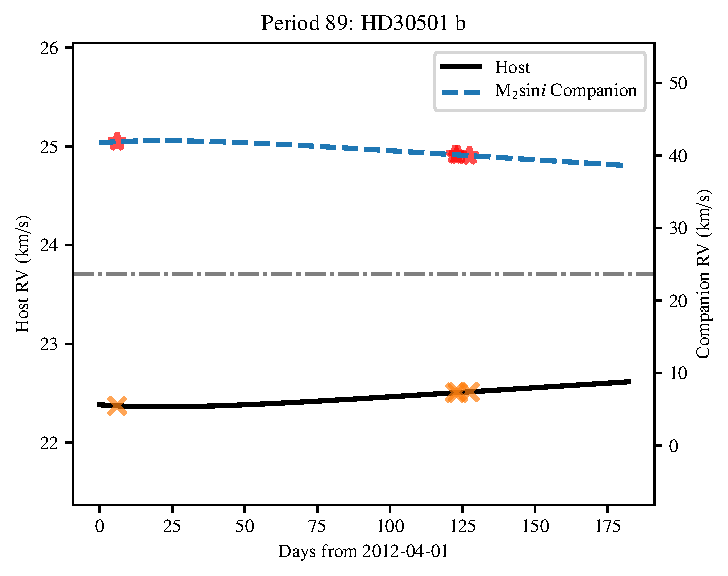
\includegraphics[width=0.45\linewidth]{figures/direct-recovery/orbital-plots/HD30501_p89.pdf}\\
    \end{tabular}
    \caption{Same as \fref{fig:hd4747p89} but for {HD\,30501}.}
    \label{fig:hd30501p89}
\end{figure}

\todo{Check M2sini labels - can we get M2 only for those that we know}

\todo{Should RV of companion be scale by m2sini only or m2 if known?}
